\chapter{Computational Model} \label{model}

\newcommand{\numcategories}[0]{$cat$ }
\newcommand{\numsubcategories}[0]{$cat$ }
\newcommand{\numsensors}[0]{$N_S$ }
\newcommand{\numstakeholders}[0]{$N_{DC}$ }
\newcommand{\numcontexts}[0]{$N_C$ }
\newcommand{\numquestions}[0]{$N_{DR}$ } 


\let\subcaption\relax
\let\subfloat\relax

\section{Introduction}
Why the model is needed, add some previous paper about incentives and what we do differently
Our aim is to create a computational model that is able to collect useful data about the influence of incentives on mobile
data sharing. (Quote some studies that have done similar studies with no data incentives). 
In the model, what we try to do is first create a user profile by asking the user some preliminary questions. Then, we proceed to assign each sensor data request
with a maximum achievable credit using the formulated user profile. The idea of the model is that it assigns requests where the user
least desires to share mobile sensor data with higher incentive costs. Respectively, the data requests where the user desires to share data more
are assigned lower incentive costs. This permits us to see whether incentives do indeed make a difference in
data sharing, since assigning more credit to data requests where the user would anyway give mobile sensor data is futile to our goals. The model aims to collect useful data that examine the relationship between incentives and mobile data sharing, mainly when the user least desires to share data.

\section{Model Intricacies}

\begin{figure}[ht!]
\centering
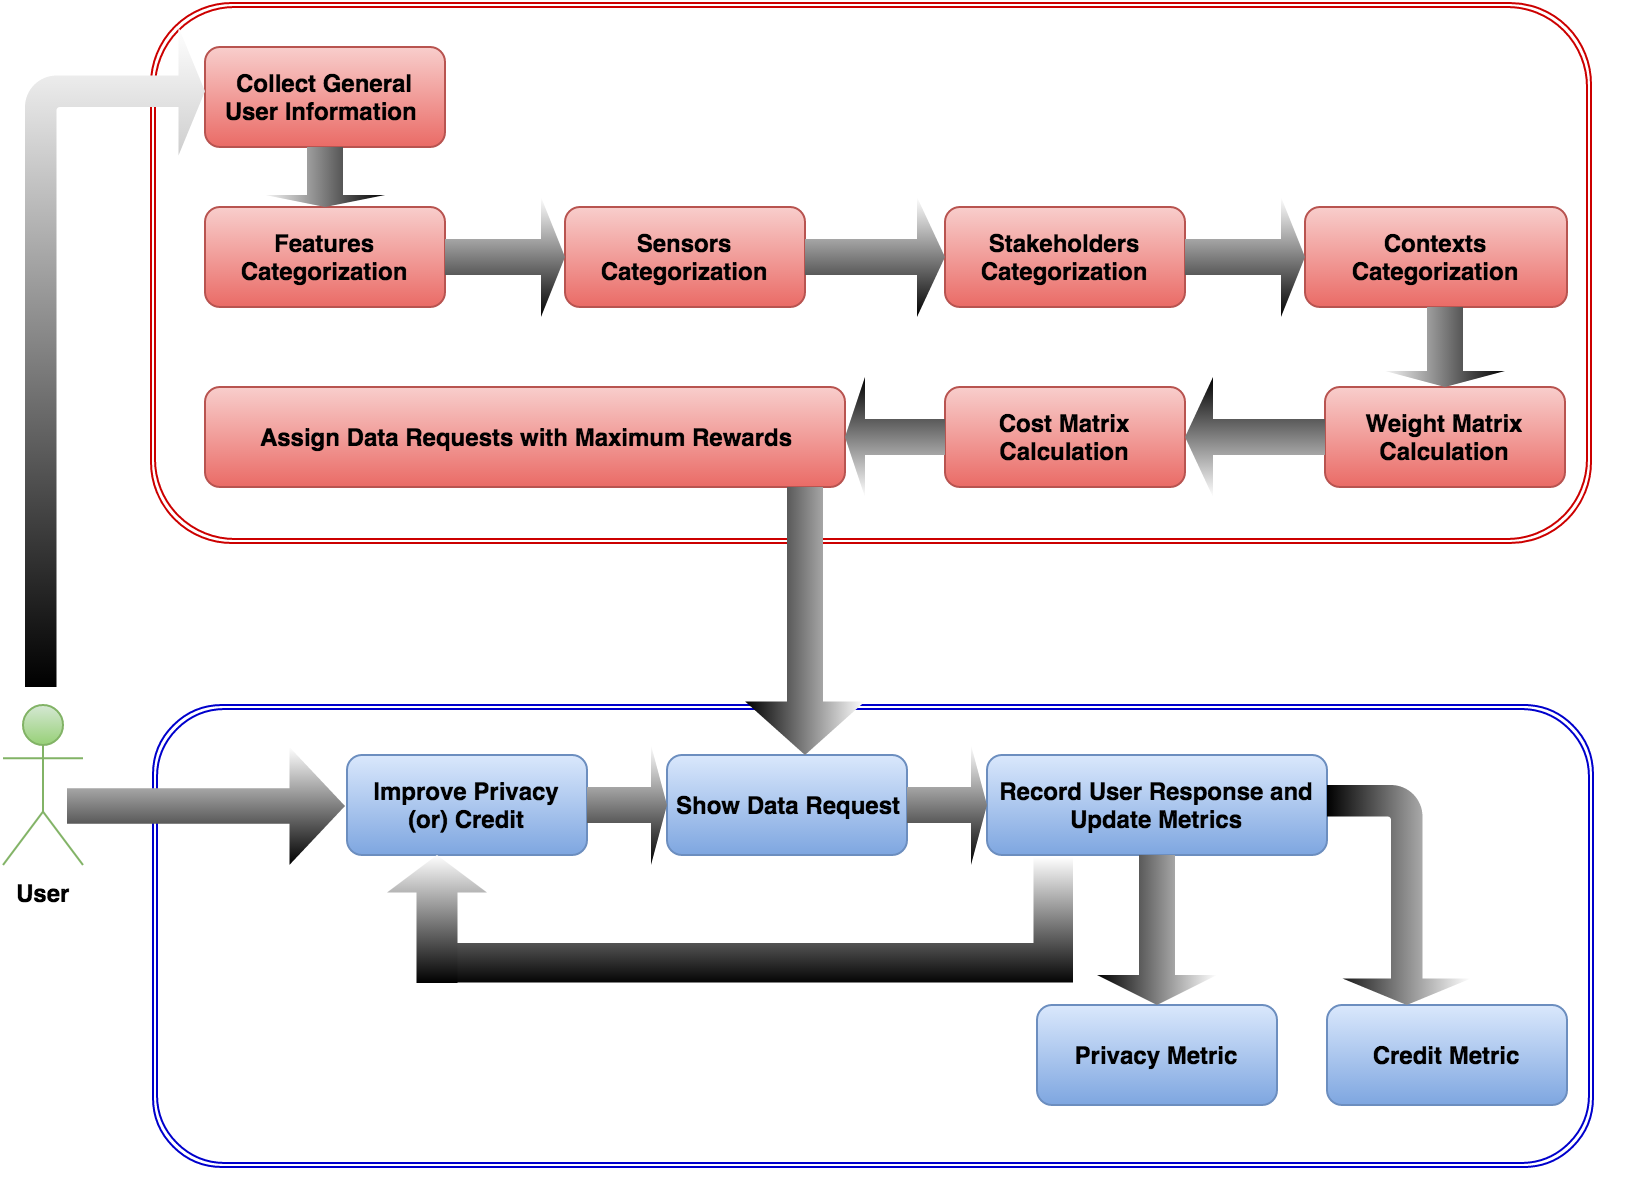
\includegraphics[width=\textwidth,keepaspectratio]{./images/model_building_blocks}
\caption{Computational Model Flow Chart \label{model_blocks}}
\end{figure}

The sections below explain the various building blocks of the computational model. The Figure \ref{model_blocks}
provides an overview of how the model works.
To begin with the model, each user is asked to enter various non-intrusive personal information that can help in analysing
the user's behavior. For example, this can consist of the age, gender, country of residence and employment.

\subsection{Categorization of the Features} \label{catfeatures}
After we are  done recording the user's personal information, we go into the categorization of the features.
In this model, features consist of Sensors, Stakeholders and Contexts. The Sensors consist of the sensors in the mobile phone which the user's
can trade. Let the category assigned to the Sensors be represented by $S$. The Stakeholders
consist of any entity that can request the user for mobile sensor data. Let the category assigned to the Sensors be represented by $DC$. The Contexts consist of the purpose for which a Stakeholder would like to obtain the user's mobile sensor data. Let the category assigned to the Sensors be represented by $C$. 
Categorization of the features means that the user places each of the features into predefined categories, and 2 or more features can
be placed into the same category. 
The user is asked to categorize each feature in the available \numcategories number of categories.
The first category indicates that the feature does not contribute much to the data sharing decision. Respectively, the category \numcategories indicates that
the feature contributes a lot to the data sharing decision. The categories are linearly scaled and equally spaced. The reason categorization was chosen is as to not rule out the possibility to that two features may be considered equally important in the data sharing decision and this may be missed by ranking the features.
Once the user has categorized the Sensors, Stakeholders and the Contexts, the weights of each feature in the data sharing decision is calculated.
The category feature Sensors has been placed into be represented by $S$, the category feature Stakeholders has been placed into be represented by $DC$ and the category feature Context has been placed into be represented by $C$. Hence the respective weights $weight_S$, $weight_{DC}$ and $weight_C$ are calculated as follows :

\begin{equation}
   weight_S = \frac{S}{S+DC+C} 
\end{equation}
\begin{equation}
   weight_{DC} = \frac{DC}{S+DC+C} 
\end{equation}
\begin{equation}
   weight_C = \frac{C}{S+DC+C} 
\end{equation}


\subsection{Categorization of the Sub-Features}
Once the features have been categorized and their weights calculated, the sub-features need to be categorized. In this model, sub-features consist
of the various types of Sensors available on the mobile phone, the various types Stakeholders that request mobile data from users and the different types of Contexts for which mobile data is requested. In other words, sub-features are the different kinds of features that appear during data request to the user. The following are examples of sub-features for each feature :

\begin{itemize}
\item Sensors : Accelerometer, Battery and Gyroscope
\item Stakeholders : Company, Non-Governmental Organization and Government.
\item Contexts : Education, Entertainment and Navigation.
\end{itemize}

\begin{figure}[ht!]
\centering
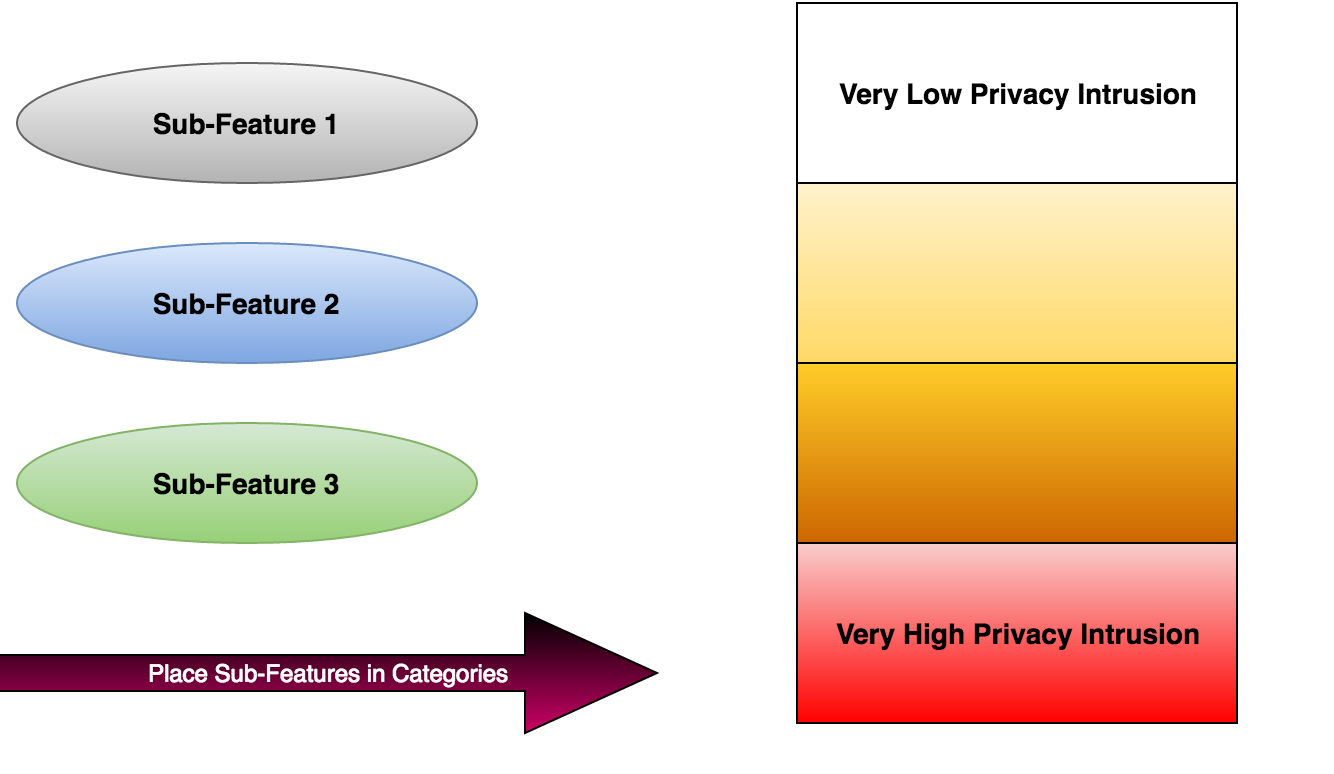
\includegraphics[width=\textwidth,keepaspectratio]{./images/categorize_sub}
\caption{Categorizing Sub-Features according to the perceived Intrusion Level \label{categorize_sub}}
\end{figure}

For each of the features, the respective sub-features are assigned a unique identifier ranging from one to the length of sub features.
Now for each of the features, the respective sub-features need to be in turn categorized in a similar fashion to section \ref{catfeatures}.
Each sub-feature can be placed in the available \numsubcategories categories. The first category indicates that the user finds the sub-feature very
non privacy intrusive. This means that the user would not be worried trading data for this sub-feature. The last category indicates that the user finds this sub-feature very privacy intrusive. This in turn means that the user would be reluctant giving data for this sub-feature. All the categories in between are linearly scaled and equally spaced.
The user then places for each feature, the respective sub-features in the \numsubcategories available categories according to the perceived
intrusion level. A conceptual diagram is shown in figure \ref{categorize_sub}. 
For the sub-features of Sensors, categories they are placed in are represented by $S_{i}$, where $S$ is the feature Sensors and $i$ is the id
of the sub-feature. Similarly, categories assigned to sub features of features Stakeholders and Contexts respectively are represented by $DC_{j}$ and $C_{k}$, where $j$ and $k$ are the id's of the sub-features categorized.




\subsection{Weight Matrix Calculation}
Each data request to the user consists of the 3 features in them. Each of those features has a number of sub-features that can appear in turns in a data request, that is in a factorial form. Let $count(feature)$ be function that gives the number of sub-features given a feature. The total number
of data requests is :

\begin{equation}
N_{DR} =  count(Sensors) * count(Stakeholders) * count(Contexts)    
\end{equation}

Let $WM$  be a matrix with dimensions $count(Sensors) x count(Stakeholders) x count(Contexts)$. We call this the weight matrix.
The cell $WM_{i,j,k}$ represents the data request which involves the Sensor's sub-feature with identifier $i$, Stakeholder's sub-feature with identifier $j$,
and the Context's sub-feature with identifier $k$. That is, each cell of $WM$ represents a data request to the user. The aim of the weight matrix is to use the information collected from the user profiling to assign various weights to each data requests. Intuitively, the process examines the
data requests where the user is least likely to trade data and assigns higher weights to those data requests. This process can be seen in
section \ref{analysis_model} in more detail. As mentioned before, each cell of the matrix $WM$ represents the weight of a data request with a unique Sensors sub-feature $i$, Stakeholders sub-feature $j$ and Contexts sub-feature $k$. To calculate the weight of a data request :

\begin{equation}
WM_{i,j,k} = (S*S_{i}) + (DC*DC_{j}) + (C*C_{k})
\end{equation}

Applying this formula to every cell gives the weight matrix $WM$.

\subsection{Cost Matrix Calculation}

Now that the weights for every data request has been calculated, we need to calculate the exact amount of money
the users can receive for a data request. Let $CM$ be the cost matrix with dimensions $count(Sensors) x count(Stakeholders) x count(Contexts)$.
Let us assume to have a budget of B for a day, where
B can be in an actual currency or any sorts of virtual credits. For now, the budget will be referred to as credits. Each cell of the cost matrix will represent the amount of credits allocated for a particular data request for one day.
To begin with, we calculate the sum of all the cells of the weight matrix $WM$:

\begin{equation}
sum(WM) = \sum\limits_{i=1}^{count(Sensors)} \sum\limits_{j=1}^{count(Stakeholders)} \sum\limits_{k=1}^{count(Contexts)} wm_{i,j,k}
\end{equation}

where the function $sum(matrix)$ gives the sum of a matrix, in this case the weight matrix.
Let $CM_{i,j,k}$ represent the credit allocated for the data request which involves the Sensor's sub-feature with identifier $i$, Stakeholder's sub-feature with identifier $j$, and the Context's sub-feature with identifier $k$. To calculate one cell of the cost matrix :

\begin{equation}
CM_{i,j,k} = \frac{WM_{i,j,k} * B}{sum(WM)}
\end{equation}

Doing this for every cell of $CM$, the whole cost matrix can be calculated. Now, we have the credits allocated per day for every data
request.

\subsection{Cost and Privacy Metrics}
Every data request now has an associated cost. This is the maximum cost that a user can obtain for that data request.
The Cost metric is the total amount of credits the user has obtained for one day. Similarly, the Privacy metric is the amount of
privacy percentage the user has maintained. That is, it intuitively quantifies the amount of data the user has refused to share hence implying privacy. The Cost and Privacy are inversely proportional to each other, in the sense that when the Cost goes up and Privacy goes down and vice versa.
For each data request, the user can choose how much data is to be shared, from the maximum amount of data to no data at all. Each option corresponds to a summarization level explained in detail in section \ref{summa}. The cost assignment to each option is linearly scaled according
to the cost assigned to each data request. Let us assume there are options for a data request ranging from $1$ to $m$ (numeric options), where $1$ corresponds to where the user gives all the data requested and $m$ to where the user chooses not give any data at all. Therefore there are a total of $m$ options for a data request.
While assigning costs there are two scenarios:

\begin{itemize}
\item Assigning option costs without a participation cost.
\item Assigning option costs inclusive of a participation cost.
\end{itemize}

Let us examine the first scenario. Let us assume that we are calculating the option costs for data request with Sensors sub-feature $i$, stakeholders sub-feature $j$ and
contexts sub-feature $k$. Let us calculate the assigned cost for option number $h$ of this data request:

\begin{equation}
cost_{h} =  \frac{CM_{i,j,k}*(m-h)}{m-1}
\end{equation}

Applying this formula by replacing $h$ by the options from $1$ to $m$ gives the cost the user receives for each option.
Similarly, if you would like to assign a participation cost to each option, it would mean that even tough the user does not share data, they still
receive some money for answering the data request. This concept can be implemented to ensure user participation. (Quote some paper with
participation of users in PSS). Let $x$ be a fraction of the total budget $B$ that is dedicated for user participation. Using a geometric progression with $a=1$ and $r=\sqrt[(m-1)]{x}$ , we can calculate the fraction of the cost $frac_{h}$ an option numbered $h$ gets:

\begin{equation}
frac_{h} = a * r^{h-1}
\end{equation}

Now that we know the fraction of the cost option $f$ can be assigned, to get the cost $cost_{h}$ of option $h$ for the data request with Sensors sub-feature $i$, stakeholders sub-feature $j$ and
contexts sub-feature $k$ :

\begin{equation}
cost_{h} = frac_{h} * CM_{i,j,k}
\end{equation}
This assigns costs to each option, taking into consideration a participation cost that the user gets even if data is not shared for that data request.

Privacy percentage $pri_{h}$ is linearly scaled between the first to the $mth$ option between $0$ and $100$ as follows:
\begin{equation}
pri_{h} = \frac{(h-1) * 100}{m-1}
\end{equation}

The total cost and privacy is the arithmetic average of all the costs and privacy obtained from every answered data request. If a data request is left unanswered, maximum privacy and minimum cost is assumed.


\subsection{Improving the Metrics}
Before the user answers a question, it is useful to know what the user interest lies in. Would the user like to improve
the privacy metric, or would the user would like to increase the credit revenue. In addition, if we know what the user is looking to improve, we can retrieve the question that can improve the that particular metric the most.
For example if the user wishes to improve his privacy further, we look at the questions where the user has given the most amount of data. We then put forth this question to answer, which indicating all the options that can improve the privacy. Similarly, if the user chooses to obtain more credit, the question where the user has given least amount of data is retrieved. Options that can improve the user credit are also indicated.


\subsection{Summarization of Collected Data} \label{summa}
As mentioned before, each data request can have options $m$ number of options the user can choose from. These options range from $1$, which indicates that the user would like to give all his data, to option number $m$, which indicates when the user does not want to give any data to this data request. Even tough all data is encrypted these days, it is still not enough as encryptions might be cracked. Summarization is a privacy algorithms that aggregates data to provide less information than in its original form. The higher the summarization level gives less data than than in its original form. The lower the summarization level gives data closer to its original form. In this model, data is collected for a period of 24 hours every $y$ seconds for every data request.If the data is summarized, according to the option chosen, the data is collected either every $y$ seconds or lesser.

Data is collected for the whole day, and at the end of the day according to the option chosen by the user, it is summarized. Summarization can
be linearly assigned to each option starting with the highest privacy corresponding to highest summarization level , that is no data sharing to
the lowest summarization level, that is no summarization at all. An example of assigning the summatization level $summ_{h}$ for option h can be the following :
\begin{equation}
summ_{h} = y*h \text{where} h \neq m
\end{equation}

This gives the frequency of sensor data collection for every option of a data request.

\section{Analysis of the Model} \label{analysis_model}
In this section, we take a scenario of the computational model and show how exactly the model works. In particular, the focus is 
on how the model varies the weights to questions according to the user input.

\subsection{Setup}
the sensors, stakeholders, and contexts and other special parameters such as number of options and all
To explain the model using examples, we take into consideration the following sub-features for each feature:

\begin{enumerate}
    \item Sensors
    \begin{enumerate}
    \item Accelerometer -1
    \item Noise -2
    \item Location -3
   \end{enumerate}
    \item Stakeholders 
    \begin{enumerate}
    \item Corporation -1
    \item Government -2
    \item education -3
   \end{enumerate}
   \item Contexts
    \begin{enumerate}
    \item Navigation -1
    \item Environment -2
    \item Social Media -3
   \end{enumerate}
 \end{enumerate}
 
The numbers indicated next to the sub-features is the sub-feature identifier. This uniquely identifies a sub-feature within a feature category.
Each user will receive an amount of $$count(Sensors)*count(Stakeholders)*count(Contexts)=27$$ data requests in total. Each data request has five privacy options ranging from one to five. the option one indicates the users would like to to trade all their data, and option five indicates the users refuse to share data their for this data request. Additionally, it is assumed that the core phase has a Budget $B=100$ per day. 
The input to the model are the user choices during the categorization of the features and sub-features.

\subsection{Results}

In this section, five user scenarios will be introduced and explained in order to explore the properties of the weight and cost matrices.
First, we will begin by introducing the way the user has categorized the features and sub-features. This will be followed by an explanation
of the generated matrices.

\subsubsection{Scenario 1 and 2}

\begin{figure}[ht!]
\centering
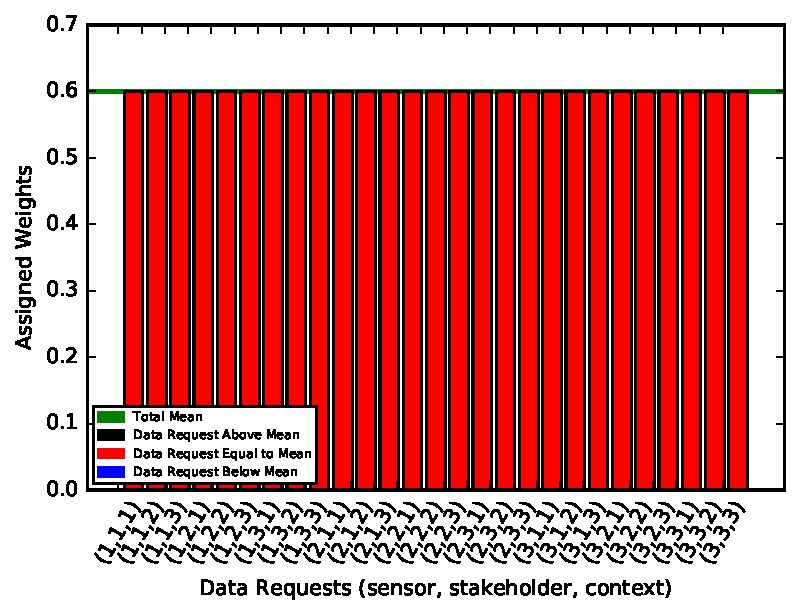
\includegraphics[width=\textwidth,keepaspectratio]{./images/weight_1_1}
\caption{Values of the Weight Matrix\label{weight11}}
\end{figure}
\begin{figure}[ht!]
\centering
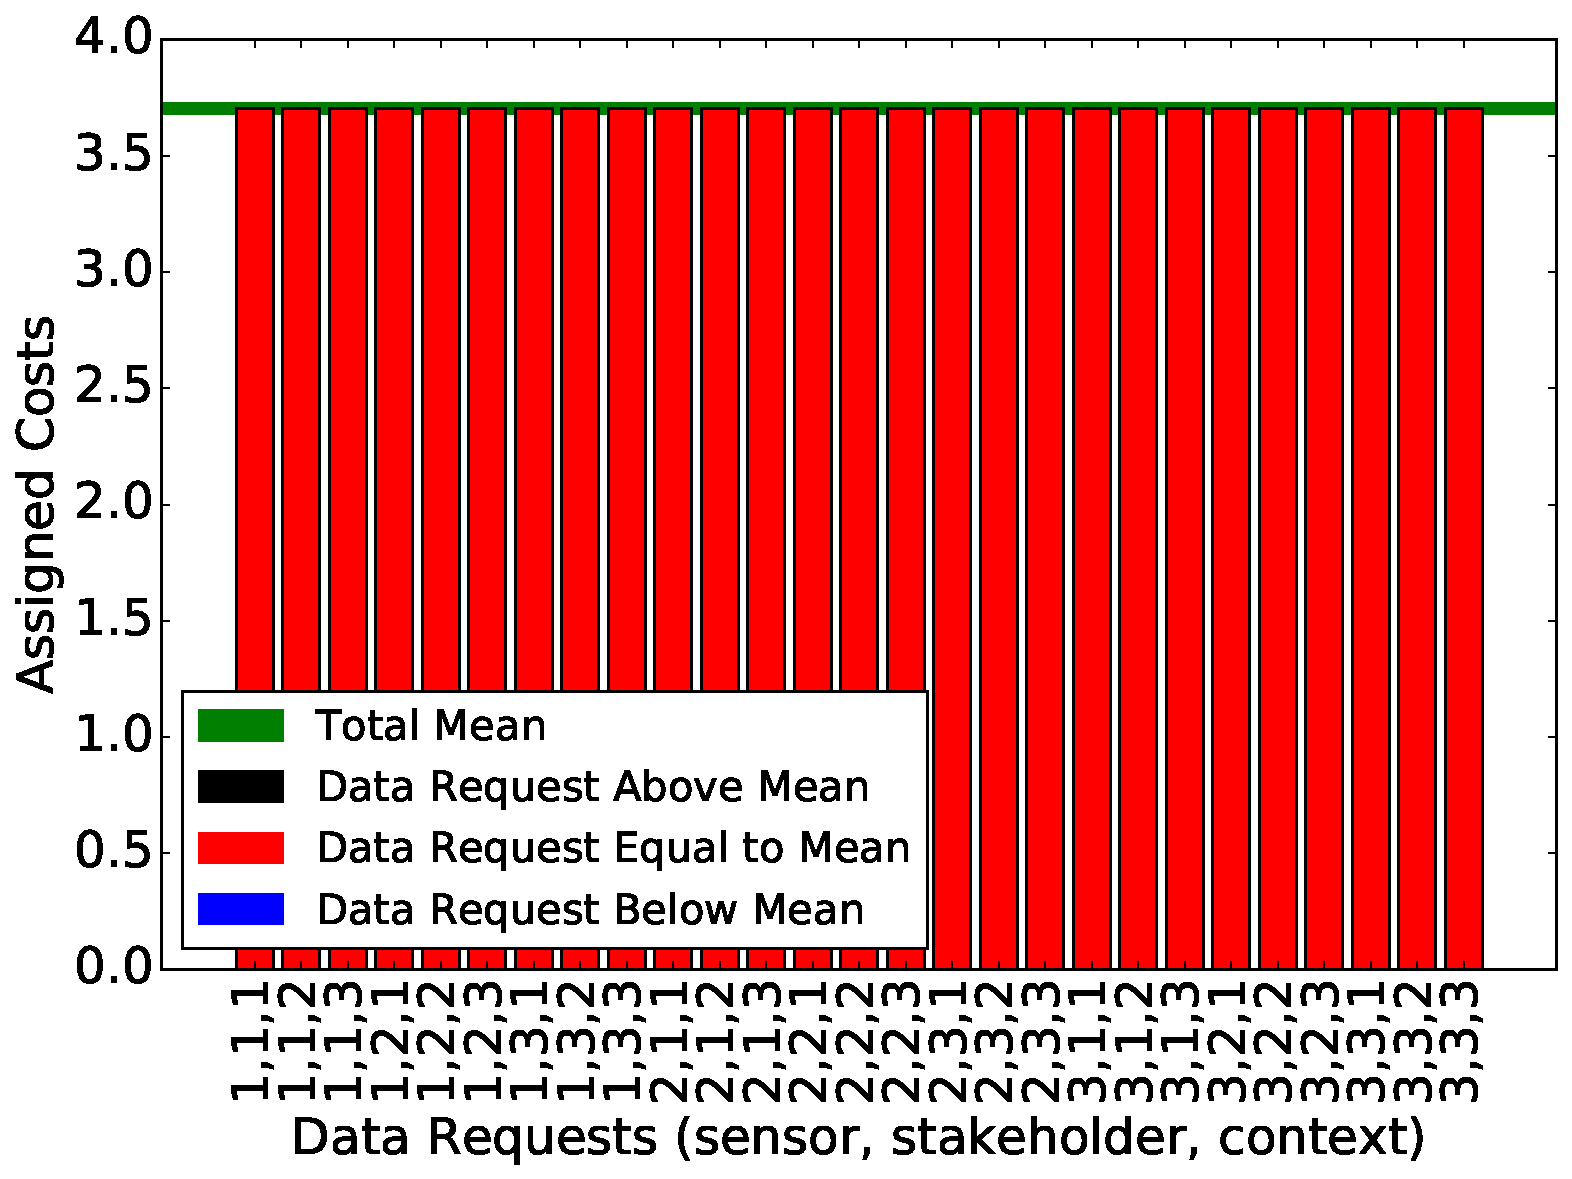
\includegraphics[width=\textwidth,keepaspectratio]{./images/cost_1_1}
\caption{Values of the Cost Matrix \label{cost11}}
\end{figure}
   






